\chapter{Labeled Hypercube}

Generalmente, in un contesto reale si cuole costruire reti che abbiano le seguenti proprietà:
\begin{itemize}
    \item \textbf{Diametro piccolo}, $O(1)$ oppure PolyLog$(n)$, in modo da ridurre i tempi di comunicazione tra i nodi.
    \item \textbf{Grado piccolo}, in modo da ottenre grafi \textbf{sparsi}, che sono più facili da costruire e mantenere.
\end{itemize}

Il principale vantaggio di un grafo sparso è la sua \textbf{scalabilità}, ovvero la capacità di crescere senza un aumento troppo grande del numero di link. Per esempio una \textit{clique} non è molto scalabile, perché se aggiunto un nuovo nodo, è necessario aggiungere altri $n-1$ link. Al contrario, se consideriamo un grafo a \textit{lista}, osserviamo che è facilmente scalabile, in quanto il grado di ciascun nodo è $2$, indipendentemente dal numero di nodi presenti. Tuttavia, il diametro di un grafo a lista è $O(n)$ (mentre il diametro di una clique è $O(1)$), il che lo rende poco efficiente per la comunicazione tra nodi distanti.

Quindi osserviamo che esiste un trade-off tra diametro e grado: se vogliamo un diametro piccolo, dobbiamo accettare un grado più grande, e viceversa. Un grafo ideale sarebbe quello che riesce a mantenere sia un diametro piccolo che un grado piccolo.

Consideriamo un altro esempio di grafo, il \textit{grafo a griglia}. In questo grafo, i nodi sono disposti in una \textbf{griglia bidimensionale}, e ogni nodo è connesso ai suoi vicini immediati. Il grado di ogni nodo è al massimo 4 (a meno che non si trovi ai bordi della griglia), e il diametro del grafo è $O(\sqrt{n})$, il che è un miglioramento rispetto al grafo a lista, ma ancora non è ideale.

\section{Broadcast su Labeled Hypercube}

Vogliamo quindi studiare il problema del broadcast in un grafo che abbia sia un diametro piccolo che un grado piccolo. Un esempio di tale grafo è l'\textbf{ipercubo etichettato} (labeled hypercube), che ha un diametro di $O(\log n)$ e un grado di $O(\log n)$, rendendolo una scelta interessante per la costruzione di reti scalabili ed efficienti.

Consideriamo l'insieme delle restrizioni 
\[
    R = \{\texttt{TR, BL, CN, UI, KN}\}
\]
dove \texttt{KN} è l'assunzione di \textbf{knowledge}, ovvero che ogni nodo la struttura della rete in cui si trova, ossia un \textbf{labeled hypercube} di dimensione $d$.

\subsection{Costruzione Hypercube}

\begin{definizione}[Hamming Distance]
    La \textbf{Hamming distance} tra due stringhe binarie $\bar{x}$ e $\bar{y}$ di lunghezza $d$, denotata come $h_d(\bar{x}, \bar{y})$, è il numero di posizioni in cui le due stringhe differiscono. Formalmente, se $\bar{x} = x_1 x_2 \ldots x_d$ e $\bar{y} = y_1 y_2 \ldots y_d$, allora:
    \[
    h_d(\bar{x}, \bar{y}) = |\{i : 1 \leq i \leq d, x_i \neq y_i\}|
    \]
\end{definizione}

\begin{definizione}[Labeled Hypercube]
    Definiamo la struttura \textbf{labeled hypercube} $\mathcal{H}_d$ di dimensione $d$ come un grafo $\mathcal{H}_d(V, E)$, dove:
    \begin{itemize}
        \item $V = \{0, 1\}^d \implies n = |V| = 2^d$. Ciascun nodo è univocamente identificato da una stringa (\textbf{label}) binaria di lunghezza $d$.
        \item $E = \{(\bar{x}, \bar{y}) : \bar{x}, \bar{y} \in V: h_d(\bar{x}, \bar{y}) = 1\} \implies m = |E| = \frac{n \cdot d}{2} = \frac{n \log_2n}{2}$. Due nodi sono connessi da un arco se e solo se differiscono in esattamente una posizione (ovvero, hanno un Hamming distance di 1).
        
        Inoltre, ogni arco è etichettato con l'indice della posizione in cui i due nodi differiscono. Ad esempio, se $\bar{x} = 000$ e $\bar{y} = 001$, allora l'arco tra $\bar{x}$ e $\bar{y}$ è etichettato con $3$, poiché differiscono solo nella terza posizione.
    \end{itemize}
\end{definizione}

Diremo che $\mathcal{H}_d$ è una struttura quasi sparsa, poiché il numero di archi è $O(n \log n)$, che è maggiore di $O(n)$ (struttura sparsa) ma ancora molto più piccolo di $O(n^2)$ (struttura densa).

\begin{figure}[htbp]
    \centering
    \animategraphics[autoplay,loop,width=0.8\textwidth]{20}{images/hypercube/hypercube-}{1}{280}
    \caption{Animazione di un labeled hypercube di dimensione $d=3$. Aprire con Adobe Reader oppure Okular.}
    \label{fig:hypercube}
\end{figure}

\textbf{Osservazione.} Il labeled hypercube è un grafo molto scalabile. Infatti si può estendere un ipercubo di dimensione $d$ con un altro ipercubo di dimensione $d$, semplicemente aggiungendo un arco tra i nodi analoghi dei due ipercubi.

\begin{figure}[htbp]
    \centering
    \begin{subfigure}[b]{0.3\textwidth}
        \centering
        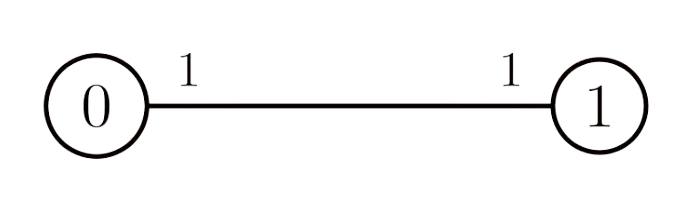
\includegraphics[width=\textwidth]{images/d1.png}
        \caption{Labeled Hypercube di dimensione $d=1$.}
        \label{fig:labelled_hypercube_d1}
    \end{subfigure}
    \hfill
    \begin{subfigure}[b]{0.3\textwidth}
        \centering
        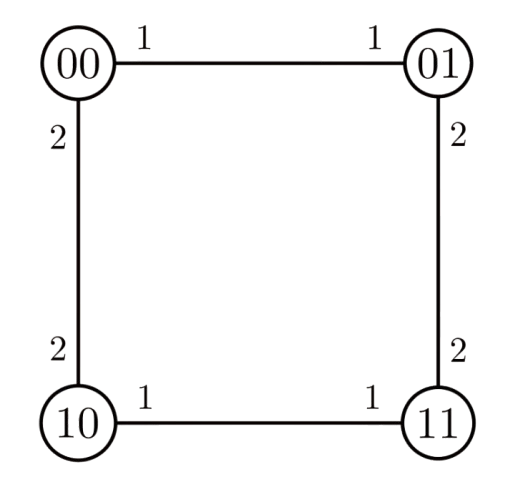
\includegraphics[width=\textwidth]{images/d2.png}
        \caption{Labeled Hypercube di dimensione $d=2$.}
        \label{fig:labelled_hypercube_d2}
    \end{subfigure}
    \hfill
    \begin{subfigure}[b]{0.3\textwidth}
        \centering
        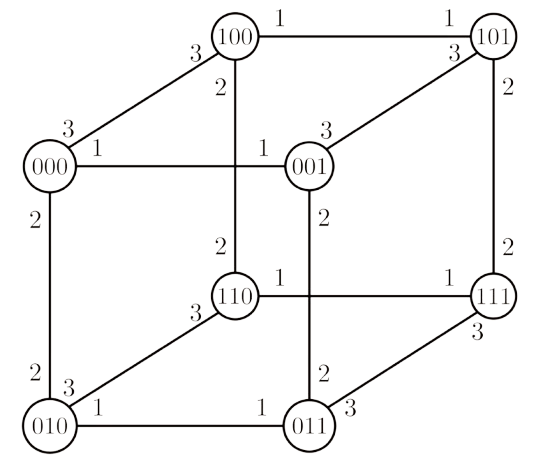
\includegraphics[width=\textwidth]{images/d3.png}
        \caption{Labeled Hypercube di dimensione $d=3$.}
        \label{fig:labelled_hypercube_d3}
    \end{subfigure}
\end{figure}

\newpage

\begin{teorema}
    Sia $\mathcal{H}_d$ un labeled hypercube di dimensione $d$. Allora:
    \begin{enumerate}
        \item $\delta(\bar{x}) = d = \log_2 n \quad \forall \bar{x} \in V$
        \item $diam(\mathcal{H}_d) = d = \log_2 n$
    \end{enumerate}
    \begin{proof}
        Dimostriamo ciascuna affermazione separatamente:
        \begin{enumerate}
            \item Poichè $|V| = 2^d$, e ogni nodo ha come vicini a distanza di hamming 1, allora ogni nodo ha esattamente $d$ vicini.
            \item Per dimostrare che il diametro è $d$, dobbiamo mostrare che $\forall \bar{x}, \bar{y} \in V$, esiste un cammino $P = (\bar{x} = \bar{v_0}, \bar{v_1}, \ldots, \bar{v_k} = \bar{y})$ tale che $k \leq d$. Siano quindi $\bar{x} = x_1 x_2 \ldots x_d$ e $\bar{y} = y_1 y_2 \ldots y_d$ due nodi arbitrari in $V$.
            \begin{itemize}
                \item Se $\bar{x} = \bar{y}$, allora $k = 0 \leq d$.
                \item Se $\bar{x} \neq \bar{y}$, scorrendo gli indici delle due stringhe a partire dalla posizione più significativa (MSB, da sinistra), e confrontando i bit, incontreremo il primo indice $j_1$ tale per cui $x_{j_1} \neq y_{j_1}$. A questo punto, per costruzione dell'ipercubo, esisterà un suo vicino $\bar{x}'$ tale che $x_{j_1}' = y_{j_1}$ e $x_i' = x_i$ per tutti gli altri indici $i$.
                \[
                    \bar{x} = x_1 x_2 \ldots x_{j_1} \ldots x_d \quad \xrightarrow{(j_1)} \quad \bar{x}' = x_1 x_2 \ldots y_{j_1} \ldots x_d
                \]
                Consideriamo quindi l'arco $(\bar{x}, \bar{x}')$ come primo arco del cammino $P$.

                A questo punto, $\forall i \leq j_1$, $x_i' = y_i$, quindi partendo dall'indice $j_1 + 1$ e continuando a scorrere verso sinistra, se arrivati a $d$ e non abbiamo ancora trovato un indice $j_2$ tale che $x_{j_2}' \neq y_{j_2}$, allora $\bar{x}' = \bar{y}$ e il cammino $P$ è completo con $k = 1 \leq d$.
                
                Altrimenti, se esiste un indice $j_2$ tale che $x_{j_2}' \neq y_{j_2}$, allora esisterà un vicino $\bar{x}''$ di $\bar{x}'$ tale che $x_{j_2}'' = y_{j_2}$ e $x_i'' = x_i'$ per tutti gli altri indici $i$.

                Iterando questo processo, alla fine si arriverà ad un nodo $\bar{x}^{(k)}$ tale che $\bar{x}^{(k)} = \bar{y}$, e il cammino $P$ sarà completo con $k \leq d$, poiché in ogni passo ci spostiamo di un bit solo, e al massimo ci sono $d$ bit da modificare per trasformare $\bar{x}$ in $\bar{y}$.
            \end{itemize}
        \end{enumerate}
    \end{proof}
\end{teorema}

\textbf{Osservazione.} Se ci spostiamo da MSB $\to$ LSB, allora il cammino $P$ che abbiamo costruito è un cammino \textbf{crescente}, ovvero un cammino in cui le etichette degli archi sono in ordine crescente. Se invece ci spostiamo da LSB $\to$ MSB, allora il cammino $P$ è un cammino \textbf{decrescente}, ovvero un cammino in cui le etichette degli archi sono in ordine decrescente.

\section{Protocollo Hyperflood}

Il protocollo \textbf{Hypercube Flooding} (Hyperflood) è un algoritmo di broadcast che sfrutta la struttura del labeled hypercube per diffondere un messaggio da un nodo sorgente a tutti gli altri nodi in modo efficiente. Inoltre, viene altamente sfruttata la conoscenza della struttura del grafo (assunzione \texttt{KN}) per ottimizzare la diffusione del messaggio.

L'idea del protocollo è la seguente: l'unico nodo $\bar{s} \in V$ \texttt{initiator} invia il messaggio $m$ a tutti i suoi vicini. Qualsiasi altro nodo $\bar{x} \neq \bar{s}$ riceve il messaggio da un arco etichettato con $l$, allora inoltrerà il messaggio su tutti gli archi 
\[
    \{(\bar{x}, \bar{y}) \in E : l' = \lambda(\bar{x}, \bar{y}) < l\}
\]

\textbf{Osservazione.} Il protocollo sfrutta la struttura gerarchica del labeled hypercube: il nodo iniziatore invia il messaggio ad un nodo all'interno di ogni sotto-ipercubo di dimensione $l' = l - 1$, e ognuno di questi nodi diventa iniziatore del sotto-ipercubo di cui fa parte.

\begin{algorithm}[H]
\caption{Hyperflood}
    \begin{algorithmic}
    \If{state($\bar{x}$) = state($\bar{s}$)} spontaneamente
        \ForAll{$\bar{y} \in N(\bar{x})$}
            \State send($m$, $\bar{y}$)
        \EndFor
    \Else
        \State $\texttt{m}, \texttt{l} \gets$ receive()
        \ForAll{$\bar{y} \in N(\bar{x})$}
            \If{$\lambda(\bar{x}, \bar{y}) < l$}
                \State send($m$, $\bar{y}$)
            \EndIf
        \EndFor
    \EndIf
    \end{algorithmic}
\end{algorithm}

\begin{teorema}[Correttezza]
    Per ogni coppia di nodi $\bar{x}, \bar{y} \in V$, esiste sempre un cammino $P$ con \textbf{etichette decrescenti} da $\bar{x}$ a $\bar{y}$. Nel protollo Hyperflood, il messaggio verrà inoltrato lungo questo cammino.
    \begin{proof}
        La dimostrazione è la stessa del secondo punto del teorema precedente, in quanto il protocollo Hyperflood costruisce esattamente un cammino con etichette decrescenti da $\bar{x}$ a $\bar{y}$.

        Vediamo invece un esempio pratico. Considerimo due nodi $\bar{x} = 100010100$ e $\bar{y} = 110001000$. Consideriamo la procedura per costruire un cammino usata nel secondo punto del teorema precedente, ma partendo da LSB $\to$ MSB, in modo da ottenere un cammino con etichette decrescenti. Consideriamo inoltre gli indici ordinai in modo decresente, allora i due nodi differiscono in posizioni $8, 5, 4, 3$. Allora, un cammino che li collega è formato dagli archi con etichette $8, 5, 4, 3$, ovvero con etichette decrescenti.
        
        \begin{figure}[htbp]
        \centering
        \animategraphics[autoplay,loop,width=0.8\textwidth]{20}{images/correttezza/hypercube-}{1}{280}
        \caption{Animazione costruzione cammino. Aprire con Adobe Reader oppure Okular.}
        \label{fig:correttezza_hyperflood}
    \end{figure}    
    \end{proof}
\end{teorema}

\begin{teorema}[Message Complexity]
    \[
        M[\texttt{Hyperflood}] = n - 1 =  O(n)
    \]
    \begin{proof}
        Per dimostrare che il numero di messaggi è $n - 1$, ossia uno per ogni nodo, mostreremo che il grafo indotto dai archi lungo cui viene trasmesso il messaggio è un \textbf{albero}.

        Supponiamo per assurdo che esiste un nodo $\bar{y}$ che riceve due copie del messaggio. Allora nel grafo delle comunicazioni esistono due cammini \textit{disgiunti} che partono da un nodo $\bar{x}$ (sorgente inclusa) e arrivano a $\bar{y}$.

        Per costruzione dell'ipercubo, i due cammini sono tali per cui i loro rispettivi archi iniziali posseggono due etichette $l_1 \neq l_2$. Senza perdità di generalità, assumiamo $l_1 < l_2$ e che l'arco a sinistra inizi con l'arco etichettato $l_1$ e quello a destra inizi con l'arco etichettato $l_2$. Sia $\bar{x}'$ il nodo raggiunto da $l_1$ e $\bar{x}''$ il nodo raggiunto da $l_2$, come in \autoref{fig:hyperflood_msg_combined}.

        \begin{figure}[ht!]
            \centering
            \begin{subfigure}[b]{0.32\textwidth}
                \centering
                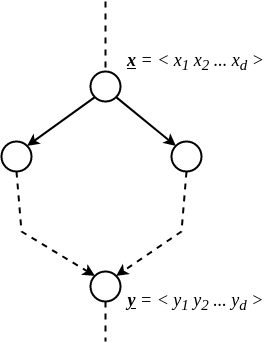
\includegraphics[width=\textwidth]{images/hyperflood_msg_1.png}
                \caption{Due cammini da $\bar{x}$ a $\bar{y}$.}
                \label{fig:hyperflood_msg_1}
            \end{subfigure}
            \hfill
            \begin{subfigure}[b]{0.32\textwidth}
                \centering
                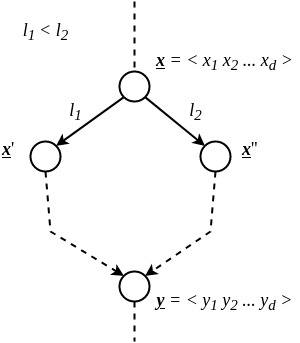
\includegraphics[width=\textwidth]{images/hyperflood_msg_2.png}
                \caption{Archi etichettati $l_1$ e $l_2$.}
                \label{fig:hyperflood_msg_2}
            \end{subfigure}
            \begin{subfigure}[b]{0.32\textwidth}
                \centering
                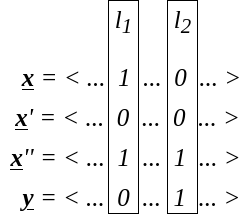
\includegraphics[width=\textwidth]{images/hyperflood_msg_3.png}
                \caption{Posizione dei bit in cui differiscono $\bar{x}$ e $\bar{y}$.}
                \label{fig:hyperflood_msg_3}
            \end{subfigure}
            \caption{Dimostrazione della struttura ad albero nel protocollo Hyperflood.}
            \label{fig:hyperflood_msg_combined}
        \end{figure}

        Per costruzione del cammino, il nodo $\bar{x}$ differisce da $\bar{y}$ almeno per i bit in posizione $l_1$ e $l_2$ (vedere animazione in \autoref{fig:correttezza_hyperflood}).

        Abbiamo quindi che $\bar{x}'$ differisce da $\bar{y}$ per il bit in posizione $l_2$, e $\bar{x}''$ differisce da $\bar{y}$ per il bit in posizione $l_1$. 

        Ci troviamo quindi nella situazione in \autoref{fig:hyperflood_msg_3}. Poiche i cammini procedono per etichette \textbf{decrescenti}, il cammino di sinistra includerà solo i nodi che differiscono da $\bar{x}'$ per i bit in posizione $l_i < l_1$, ma questo implica che il cammino di sinistra porta a $\bar{y}$ senza mai cambiare il bit in posizione $l_2$, ma questo è un \textbf{assurdo} dato che $\bar{x}$ e $\bar{y}$ differiscono per il bit in posizione $l_2$.

        Questo dimostra che nel grafo di comunicazione non ci sono cicli, e quindi è un albero. Di conseguenza, ogni nodo riceve esattamente un messaggio, e il numero totale di messaggi è $n - 1$.
    \end{proof}
\end{teorema}

\begin{teorema}[Ideal Time]
    Sotto le restrizioni 
    \[
    R \cup \{\texttt{Synchronized Clock, Bounded Communication Delay}\}
    \]
    il tempo ideale per il broadcast è $O(\log n)$.
    \begin{proof}
        Dimostrazione per induzione sulla \textit{distanza di Hamming} dei nodi dalla sorgente. Dimostriamo che per ogni $j \geq d$, e per ogni $\bar{x}$ a distanza di Hamming $j$ dalla sorgente, il nodo $\bar{x}$ riceve il messaggio al tempo $j$.

        \[
            \forall j \in [d], \forall \bar{x} \in V = \{0, 1\}^d: h_d(\bar{s}, \bar{x}) = j \implies t_{recv}(\bar{x}) = j
        \]
        Per $j = 1$ è banale, in quanto per definizione del protocollo, la sorgente invia il messaggio a tutti i suoi vicini i quali hanno distanza di Hamming 1 dalla sorgente, e quindi ricevono il messaggio al tempo $t = 1$.

        Definiamo ora $L_j = \{ \bar{x} \in V : h_d(\bar{s}, \bar{x}) = j \}$ e supponiamo per induzione che sia vero per $j - 1$, ovvero che tutti i nodi in $L_{j-1}$ ricevano il messaggio al tempo $t = j - 1$. Sappiamo che per ogni nodo $\bar{x} \in L_j$, esiste un cammino con etichette decrescenti da $\bar{s}$ a $\bar{x}$, allora esiste un nodo $\bar{y} \in L_{j-1}$ tale che $\bar{x}$ è un vicino di $\bar{y}$. Per ipotesi, $\bar{y}$ è già stato informato al tempo $t = j - 1$ e inoltre il messaggio impiega un istante per attraversare l'arco $(\bar{y}, \bar{x})$, quindi $\bar{x}$ riceve il messaggio al tempo $t = j$. 
        Poiché la lunghezza massima di un cammino è $d$, allora ogni nodo riceve il messaggio al tempo $t \leq d = O(\log n)$.
    \end{proof}
\end{teorema}